% !TeX encoding = UTF-8
% !TeX program = XeLaTeX
% !TeX spellcheck = LaTeX

\documentclass[a4paper]{article}

\usepackage{amsmath,amsfonts,amssymb}
\usepackage{mathrsfs}
\usepackage{bm}
\usepackage{extarrows}
\usepackage{geometry}
\usepackage{ntheorem}
\usepackage{hyperref}
\usepackage[ruled]{algorithm2e}
\usepackage{caption,subcaption}
\usepackage{tikz}

\usetikzlibrary{automata}

\geometry{left=2cm,right=2cm,top=2cm,bottom=2cm}

\def\UrlBreaks{\do\A\do\B\do\C\do\D\do\E\do\F\do\G\do\H\do\I\do\J\do\K\do\L\do\M\do\N\do\O\do\P\do\Q\do\R\do\S\do\T\do\U\do\V\do\W\do\X\do\Y\do\Z\do\[\do\\\do\]\do\^\do\_\do\`\do\a\do\b\do\c\do\d\do\e\do\f\do\g\do\h\do\i\do\j\do\k\do\l\do\m\do\n\do\o\do\p\do\q\do\r\do\s\do\t\do\u\do\v\do\w\do\x\do\y\do\z\do\0\do\1\do\2\do\3\do\4\do\5\do\6\do\7\do\8\do\9\do\.\do\@\do\\\do\/\do\!\do\_\do\|\do\;\do\>\do\]\do\)\do\,\do\?\do\'\do+\do\=\do\#}

\newtheorem{theorem}{Theorem}
\newtheorem{lemma}{Lemma}
\newtheorem{proposition}{Proposition}
\newtheorem{corollary}{Corollary}
\newtheorem{claim}{Claim}
\newtheorem{conjecture}{conjecture}
\newtheorem{definition}{Definition}
\newtheorem{construction}{Construction}
\newtheorem*{proof}{Proof}
\newtheorem*{answer}{Answer}
\newtheorem*{example}{Example}
\newtheorem*{counterexample}{Counterexample}

\newenvironment{exercise}[1]{
	\par
	\noindent\textbf{Exercise #1.}\quad
}{
	\par
	\bigskip
}
\newenvironment{problem}[1]{
	\par
	\noindent\textbf{Problem #1.}\quad
}{
	\par
	\bigskip
}

\DeclareMathAccent{\widehat}{\mathord}{largesymbols}{"62}
\DeclareMathOperator*{\argmax}{\arg\,\max}
\DeclareMathOperator*{\argmin}{\arg\,\min}
\DeclareMathOperator{\E}{\mathbb E}
\DeclareMathOperator{\Var}{\mathrm{Var}}
\DeclareMathOperator{\tr}{\mathrm{tr}}
\DeclareMathOperator{\poly}{\mathrm{poly}}
\newcommand{\abs}[1]{\left| #1 \right|}
\newcommand{\vabs}[1]{\left\| #1 \right\|}
\newcommand{\abra}[1]{\left\langle #1 \right\rangle}
\newcommand{\pbra}[1]{\left( #1 \right)}
\newcommand{\cbra}[1]{\left\{ #1 \right\}}
\newcommand{\sbra}[1]{\left[ #1 \right]}
\newcommand{\floorbra}[1]{\left\lfloor #1 \right\rfloor}
\newcommand{\ceilbra}[1]{\left\lceil #1 \right\rceil}
\newcommand{\bin}{\{0,1\}}
\newcommand{\ZPP}{\mathtt{ZPP}}
\newcommand{\RP}{\mathtt{RP}}
\newcommand{\coRP}{\mathtt{co}\text{-}\mathtt{RP}}
\newcommand{\per}{\text{per}}
\newcommand{\sgn}{\text{sgn}}
\newcommand{\Fbb}{\mathbb{F}}
\newcommand{\Nbb}{\mathbb{N}}
\newcommand{\Rbb}{\mathbb{R}}
\newcommand{\Zbb}{\mathbb{Z}}
\newcommand{\Sset}{\mathbb{S}}
\newcommand{\Fset}{\mathbb{F}}
\newcommand{\Nset}{\mathbb{N}}
\newcommand{\Zset}{\mathbb{Z}}
\newcommand{\Uset}{\mathbb{U}}
\newcommand{\Acal}{\mathcal{A}}
\newcommand{\Bcal}{\mathcal{B}}
\newcommand{\Ccal}{\mathcal{C}}
\newcommand{\Fcal}{\mathcal{F}}
\newcommand{\Gcal}{\mathcal{G}}
\newcommand{\qd}[2]{{\left(\frac{#1}{#2}\right)}}
\newcommand{\dv}{\ |\ }
\newcommand{\mylm}{\xLongrightarrow[lm]{}}
\newcommand{\myrm}{\xLongrightarrow[rm]{}}

\bibliographystyle{plainnat}

\title{Exercise Set --- Chapter $8$}
\date{}

\begin{document}

\maketitle

\noindent\textbf{Notation:}
\begin{itemize}
\item If $w$ is a string, then $w[i]$ stands for the $i$-th character in $w$.
\item In $k$-tape Turing Machine, $T_i$ represents the $i$-th tape.
\end{itemize}

\begin{exercise}{8.2.2} \hspace{0pt}\\
\textbf{a)} $L=\{w\in\{0,1\}^*|c_0(w)=c_1(w)\}$.
    \begin{center}
    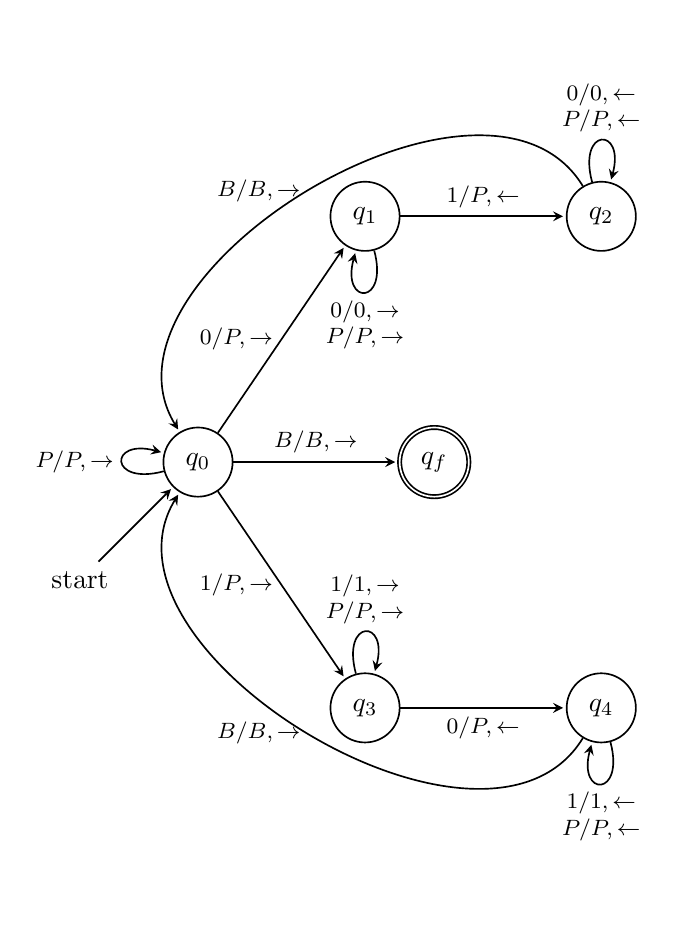
\begin{tikzpicture}[shorten >=1pt,->,>=stealth,semithick,node distance=3cm,auto,align=center]
        \node[state] (q0) {$q_0$};
        \node (f) at (-1.5,-1.5) {start};
        \draw[->] (f) -- (q0);
        \node[state] (q1) [above right of=q0,yshift=1cm] {$q_1$};
        \node[state] (q2) [right of=q1] {$q_2$};
        \node[state] (q3) [below right of=q0,yshift=-1cm] {$q_3$};
        \node[state] (q4) [right of=q3] {$q_4$};
        \node[state,accepting] (qf) [right of=q0] {$q_f$};

        \footnotesize
        \path[->] (q0) edge [loop left] node {$P/P,\rightarrow$} ()
                       edge node [above] {$B/B,\rightarrow$} (qf)
                       edge node [left] {$0/P,\rightarrow$} (q1)
                       edge node [left] {$1/P,\rightarrow$} (q3)
                  (q1) edge [loop below] node {$0/0,\rightarrow$\\$P/P,\rightarrow$} ()
                       edge node [above] {$1/P,\leftarrow$} (q2)
                  (q2) edge [loop above] node {$0/0,\leftarrow$\\$P/P,\leftarrow$} ()
                       edge [bend right=90] node [left] {$B/B,\rightarrow$} (q0)
                  (q3) edge [loop above] node {$1/1,\rightarrow$\\$P/P,\rightarrow$} ()
                       edge node [below] {$0/P,\leftarrow$} (q4)
                  (q4) edge [loop below] node {$1/1,\leftarrow$\\$P/P,\leftarrow$} ()
                       edge [bend left=90] node [left] {$B/B,\rightarrow$} (q0);
    \end{tikzpicture}
    \end{center}
\textbf{b)} $L=\{a^nb^nc^n|n\geqslant 1\}$.
    \begin{center}
    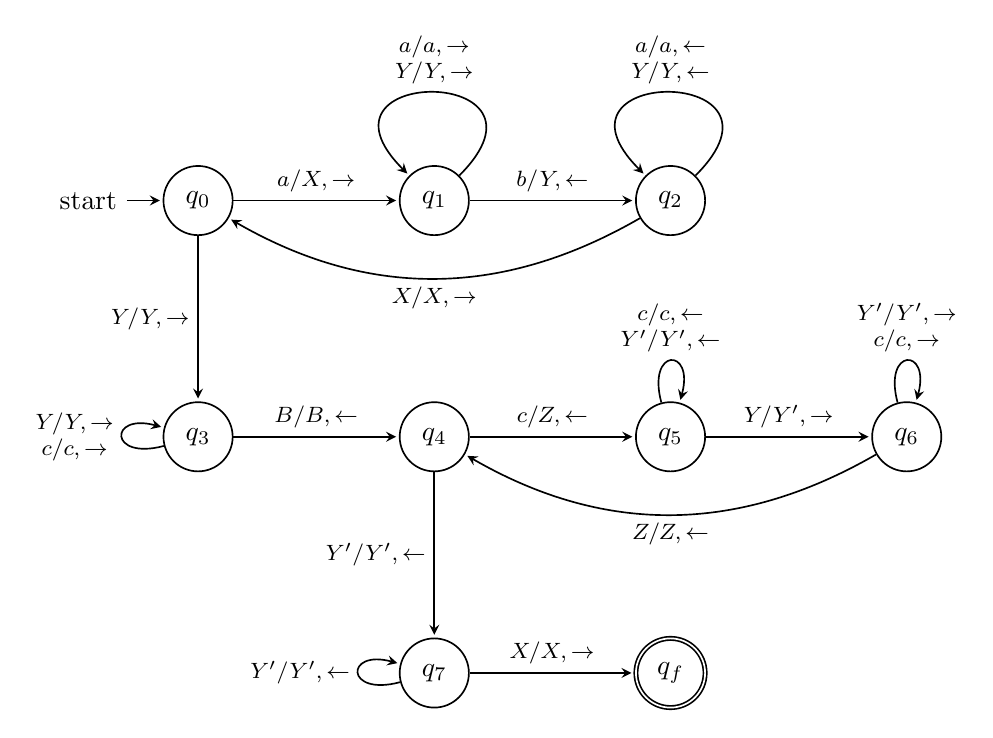
\begin{tikzpicture}[shorten >=1pt,->,>=stealth,semithick,node distance=3cm,auto,align=center]
        \node[state,initial] (q0) {$q_0$};
        \node[state] (q1) [right of=q0] {$q_1$};
        \node[state] (q2) [right of=q1] {$q_2$};
        \node[state] (q3) [below of=q0] {$q_3$};
        \node[state] (q4) [right of=q3] {$q_4$};
        \node[state] (q5) [right of=q4] {$q_5$};
        \node[state] (q6) [right of=q5] {$q_6$};
        \node[state] (q7) [below of=q4] {$q_7$};
        \node[state,accepting] (q8) [right of=q7] {$q_f$};

        \footnotesize
        \path[->] (q0) edge node [above] {$a/X,\rightarrow$} (q1)
                       edge node [left] {$Y/Y,\rightarrow$} (q3)
                  (q1) edge [loop] node [above] {$a/a,\rightarrow$\\$Y/Y,\rightarrow$} ()
                       edge node [above] {$b/Y,\leftarrow$} (q2)
                  (q2) edge [loop] node [above] {$a/a,\leftarrow$\\$Y/Y,\leftarrow$} ()
                       edge [bend left] node {$X/X,\rightarrow$} (q0)
                  (q3) edge [loop left] node {$Y/Y,\rightarrow$\\$c/c,\rightarrow$} ()
                       edge node [above] {$B/B,\leftarrow$} (q4)
                  (q4) edge node [above] {$c/Z,\leftarrow$} (q5)
                       edge node [left] {$Y'/Y',\leftarrow$} (q7)
                  (q5) edge [loop above] node {$c/c,\leftarrow$\\$Y'/Y',\leftarrow$} ()
                       edge node [above] {$Y/Y',\rightarrow$} (q6)
                  (q6) edge [loop above] node {$Y'/Y',\rightarrow$\\$c/c,\rightarrow$} ()
                       edge [bend left] node {$Z/Z,\leftarrow$} (q4)
                  (q7) edge [loop left] node {$Y'/Y',\leftarrow$} ()
                       edge node [above] {$X/X,\rightarrow$} (q8);
    \end{tikzpicture}
    \end{center}
\textbf{c)} $L=\{ww^R|w\in\{0,1\}^*\}$.
    \begin{center}
    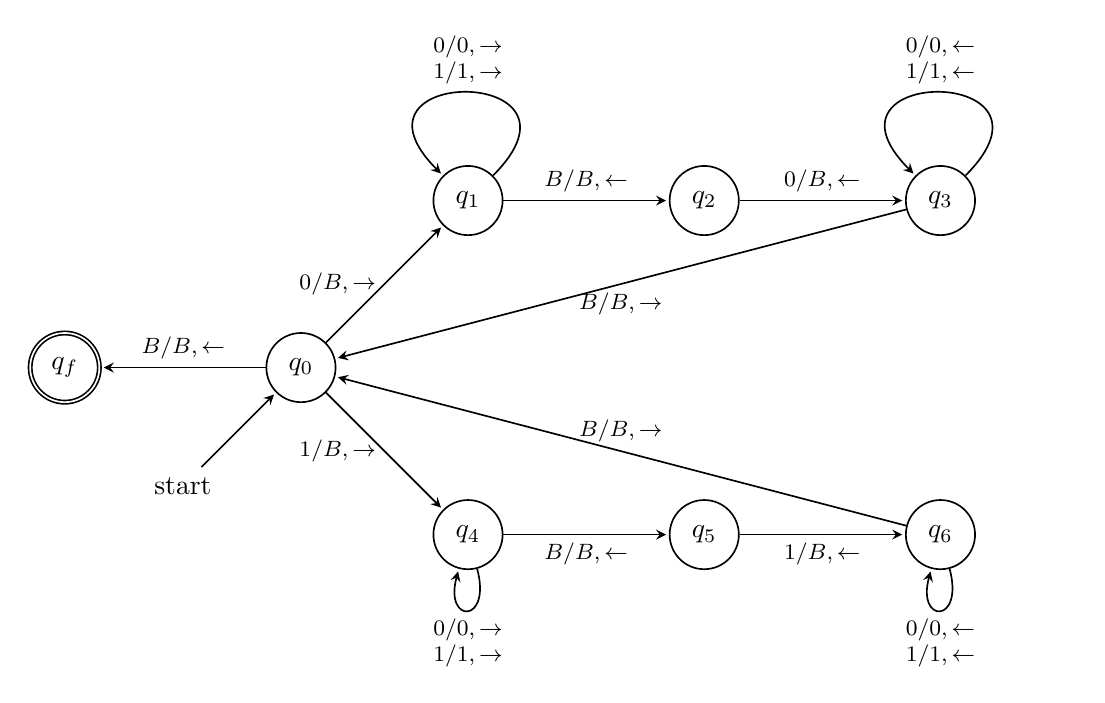
\begin{tikzpicture}[shorten >=1pt,->,>=stealth,semithick,node distance=3cm,auto,align=center]
        \node[state] (q0) {$q_0$};
        \node (f) at (-1.5,-1.5) {start};
        \draw[->] (f) -- (q0);
        \node[state] (q1) [above right of=q0] {$q_1$};
        \node[state] (q2) [right of=q1] {$q_2$};
        \node[state] (q3) [right of=q2] {$q_3$};
        \node[state] (q4) [below right of=q0] {$q_4$};
        \node[state] (q5) [right of=q4] {$q_5$};
        \node[state] (q6) [right of=q5] {$q_6$};
        \node[state,accepting] (q7) [left of=q0] {$q_f$};

        \footnotesize
        \path[->] (q0) edge node [left] {$0/B,\rightarrow$} (q1)
                       edge node [above] {$B/B,\leftarrow$} (q7)
                       edge node [left] {$1/B,\rightarrow$} (q4)
                  (q1) edge [loop] node [above] {$0/0,\rightarrow$\\$1/1,\rightarrow$} ()
                       edge node [above] {$B/B,\leftarrow$} (q2)
                  (q2) edge node [above] {$0/B,\leftarrow$} (q3)
                  (q3) edge [loop] node [above] {$0/0,\leftarrow$\\$1/1,\leftarrow$} ()
                       edge node [below] {$B/B,\rightarrow$} (q0)
                  (q4) edge [loop below] node [below] {$0/0,\rightarrow$\\$1/1,\rightarrow$} ()
                       edge node [below] {$B/B,\leftarrow$} (q5)
                  (q5) edge node [below] {$1/B,\leftarrow$} (q6)
                  (q6) edge [loop below] node [below] {$0/0,\leftarrow$\\$1/1,\leftarrow$} ()
                       edge node [above] {$B/B,\rightarrow$} (q0);
    \end{tikzpicture}
    \end{center}
\end{exercise}

\begin{exercise}{8.2.4} \hspace{0pt}\\
\textbf{a)} Assume TM $M$ computes $f$ and the input is $[x,y]$.
    Construct TM $N$ with two tapes to accept the graph of $f$:
    \begin{enumerate}
        \item Copy $x$ to the second tape
        \item Simulate $M$ on the second tape to obtain $f(x)$
        \item If $f(x)$ matches $y$, accept; otherwise, reject
    \end{enumerate}
\textbf{b)} Assume TM $N$ accepts the graph of $f$ and the input is $x$.
    Construct TM $M$ with two tapes to compute $f$:
    \begin{enumerate}
        \item Write $y$ as $0$ on the first tape
        \item Copy $[x,y]$ to the second tape
        \item Simulate $N$ on the second tape
        \item If $N$ accepts, then $y$ is $f(x)$; otherwise increase $y$ by $1$, repeat from step $2$
    \end{enumerate}
\textbf{c)} For part (a), it is partial. Because if $f$ is not defined on $x$, $N$ will never
    go to step $3$, thus never halts.\par
    For part (b), it is not partial. Because if $f(x)=1$ but $N$ will not stop when inputted $[x,0]$,
    $M$ will never get to try $y=1$. Improve this method by introducing simulation steps:
    \begin{enumerate}
        \item Write $y$ as $0$, $z$ as $0$ on the first tape
        \item Copy $[x,y]$ to the second tape
        \item Simulate $N$ for $z$ steps on the second tape
        \item If $N$ accepts, then $y$ is $f(x)$; otherwise increase $y,z$ along the diagonal
            ($0,0\to 1,0\to 0,1\to 2,0\to 1,1\to 0,2\to\cdots$), repeat from step $2$
    \end{enumerate}
\end{exercise}

\begin{exercise}{8.4.5}\hspace{0pt}\\
\textbf{a)} $M=(Q,\Sigma,\Gamma,\delta,q_0,B,F)=(\{q_0,r,p\},\{\$\},\{B,\$\},\delta,q_0,B,p)$,
    where $\delta$ is
    \begin{align*}
        \delta(q_0,\$) &=\{(r,\$,L)\}\\
        \delta(q_0,B) &=\{(q_0,B,L),(q_0,B,R)\}\\
        \delta(r,B) &=\{(p,B,R)\}.
    \end{align*}
\textbf{b)} $N=(Q,\Sigma,\Gamma,\delta,q_0,B,F)=(\{q_0,q_l,q_r,q_{ll},q_{rr},p\},\{\$\},\{B,\$,X\},\delta,q_0,B,p)$,
    where $\delta$ is
    \begin{center}
    \begin{tabular}{c|ccc}
        State & $B$ & $\$$ & $X$ \\
        \hline\hline
        $q_0$ & $(q_l,X,L)$ & --- & --- \\
        $q_l$ & $(q_r,X,R)$ & $(q_{ll},\$,L)$ & $(q_l,X,L)$ \\
        $q_{ll}$ & $(p,B,R)$ & --- & --- \\
        $q_r$ & $(q_l,X,L)$ & $(q_{rr},\$,R)$ & $(q_r,X,R)$ \\
        $q_{rr}$ & $(p,B,L)$ & --- & --- \\
        $p$ & --- & --- & --- \\
    \end{tabular}
    \end{center}
\end{exercise}

\begin{exercise}{8.4.9} Define the transition function of a $k$-head TM to be
    $$
    \delta\big((q_{t_1},q_{t_2},\cdots,q_{t_k}),c_1c_2\cdots c_k\big)=
    \big((q_{t'_1},q_{t'_2},\cdots,q_{t'_k}),c'_1c'_2\cdots c'_k,M_1M_2\cdots M_k\big),M_i\in\{L,R\},
    $$
    which means,
    if the $i$-th head reads $c_i$ in the tape at state $q_{t_i}$ respectively, then the transition
    is that the $i$-th head writes $c'_i$ in the tape, switch to state $q_{t'_i}$, and move the head based on $M_i$.
    \begin{proof}\hspace{0pt}\\
    \textbf{Ordinary} $\Rightarrow$ \textbf{$k$-head}:
        Assume ordinary TM $M=(Q,\Sigma,\Gamma,\delta,q_0,B,F)$, construct the $k$-head TM
        $N=(Q^k,\Sigma,\Gamma,\delta',(q_0,\cdots,q_0),B,F')$, where $\delta'$ is
        \begin{gather*}
        \delta'\big((q_i,q_i,\cdots,q_i),cc\cdots c\big)=\big((q_j,q_j,\cdots,q_j),c'c'\cdots c',MM\cdots M\big)\\
        \text{if }\delta(q_i,c)=(q_j,c',M),
        \end{gather*}
        and $F'=(q_f,\cdots,q_f),q_f\in F$.\par
        Then $L(N)=L(M)$.\\
    \textbf{$k$-head} $\Rightarrow$ \textbf{$3$-tape}:
        Assume $k$-head TM is $M$, construct the $3$-tape TM $N$ as follows:
        \begin{enumerate}
            \item Write down $k$ seperate zeros on $T_2$, indicating the location of $k$ heads in $T_1$
            \item Use the locations of $k$ heads on $T_2$ to find the characters under $k$ heads on $T_1$, and
                transcript them to $T_3$
            \item Use the transcripted characters on $T_3$ to simulate the transition in $M$
            \item Based on the transition, overwrite the characters under $k$ heads on $T_1$ in ascending order
            \item Based on the transition, increase or decrease the $k$ location numbers on $T_2$
            \item Repeat from step $2$
        \end{enumerate}
        When $N$ stucks in making transition, if the current state is accepting in $M$, then accept;
        otherwise, reject.\par
        Then $L(N)=L(M)$.\\
    \textbf{$3$-tape} $\Rightarrow$ \textbf{ordinary}:
        Proved in book.
    \end{proof}
\end{exercise}

\begin{exercise}{8.4.10} Define the transition function of a $2$D TM to be
    $$
    \delta(q_i,c)=(q_j,c',M),\quad M\in\{L,R,U,D\},
    $$
    where $L,R,U,D$ mean \textit{left, right, up, down} respectively.
    \begin{proof}\hspace{0pt}\\
    \textbf{Ordinary} $\Rightarrow$ \textbf{$2$D}:
        Since the transition function of ordinary TM is
        $$
        \delta(q_i,c)=(q_j,c',M),\quad M\in\{L,R\}\subset\{L,R,U,D\},
        $$
        any ordinary TM $M$ can be directly viewed as a $2$D TM $N$.\par
        Then $L(M)=L(N)$.\\
    \textbf{$2$D} $\Rightarrow$ \textbf{$3$-tape}:
        Let $f(x,y)=\frac{(x+y)(x+y+1)}{2}+y$, which is a bijection between $\Nset^2$ and $\Nset$.
        Let
        $$
        g(n)=\begin{cases}
            2n & n\geqslant 0\\
            -2n-1 & n<0
        \end{cases},
        $$
        which is a bijection between $\Zset$ and $\Nset$ and its inverse is easy to compute in a TM
        $$
        g^{-1}(n)=\begin{cases}
            \frac n 2 & n\equiv 0 \mod 2\\
            -\frac{n+1}{2} & n\equiv 1 \mod 2
        \end{cases}.
        $$
        As a result, we have $h(x,y)=g^{-1}(f(g(x),g(y)))$, a bijection between $\Zset^2$ and $\Zset$.\par
        Assume $2$D TM is $M$, construct the $3$-tape TM $N$ as follows:
        \begin{enumerate}
            \item Copy the input string on $T_1$ to $T_2$ and clear $T_1$
            \item Transcript the $i$-th character on $T_2$ to the $g^{-1}(f(g(0),g(i)))$-th cell on $T_1$;
                the calculation can be done on $T_3$
            \item Clear $T_2$
            \item Write down $(0,0)$ on $T_2$, indicating the Cartesian coordinate of the head, viz, $(x,y)$
            \item Compute $g^{-1}(f(g(x),g(y)))$ as $z$ on $T_3$ using $(x,y)$ on $T_2$
            \item Move the head in $T_1$ to the $z$-th cell
            \item Simulate $M$ to make the transition
            \item Based on the transition, overwrite the character on $T_1$ and change $(x,y)$ to $(x',y')$ on $T_2$
            \item Repeat from step $5$
        \end{enumerate}
        When $N$ stucks in making transition, if the current state is accepting in $M$, then accept;
        otherwise, reject.\par
        Then $L(N)=L(M)$.\\
    \textbf{$3$-tape} $\Rightarrow$ \textbf{ordinary}:
        Proved in book.
    \end{proof}
\end{exercise}

\begin{exercise}{8.5.1} \hspace{0pt}\\
\textbf{a)} One counter for $\{0^n1^m|n\geqslant m\geqslant 1\}$\par
    When reading $0$'s, add $1$ for every occurrence. Then read $1$'s, subtract $1$ for every occurrence until
    the counter goes to zero or the reading stops. Accept if the counter is not zero.\\
\textbf{c)} Two counter for $\{a^ib^jc^k|i=j\text{ or }i=k\}$\par
    When reading $a$'s, add $1$ for every occurrence for both counters. Then read $b$'s, subtract $1$ from first counter,
    if it is zero before subtraction, reject. Then read $c$'s, subtract $1$ from second counter,
    if it is zero before subtraction, reject.\par
    Accept if one of the counters is zero.
\end{exercise}

\end{document}
